%!TeX root=thesis.tex

\chapter{Active Learning}
\label{cha:active-learning}

In this chapter we discuss active learning and look at its application to both
the galaxy classification task and to the Radio Galaxy Zoo project. In Section
\ref{sec:intro-active-learning}, we will briefly describe the key concepts of
active learning, moving to discuss querying strategies for active learning for
binary classification in \ref{sec:query-strategies}. We apply these methods in a
simple experiment in Section \ref{sec:rgz-qbc}, showing that active learning may
be useful in an astronomical context.

Section \ref{sec:active-learning-on-crowds} extends the active learning
discussion to a crowdsourcing context, and we discuss how crowdsourcing
complicates active learning. Finally, in Section \ref{sec:al-citizen-science},
we look at the differences between the standard crowdsourcing context and
citizen science, pointing out how they differ and how this breaks assumptions of
existing methods. We end with describing an ideal experiment for active learning
applications in citizen science.

\section{Introduction}
\label{sec:intro-active-learning}
    
    In supervised learning we deal with a set of data points and their
    associated labels. This dataset may be expensive to obtain, but the main
    costs may come from collecting labels, rather than from collecting the data
    points themselves. Examples of such data include text samples
    \citep{lewis94, mccallum98}, and images \citep{loy11, lintott08}, both of
    which are now widely and cheaply available through the internet. A more
    abstract example is scientific hypotheses \citep{king04}. Labelling text and
    images is hard, error-prone, and requires humans; and performing a
    scientific experiment to test a hypothesis is considerably more expensive
    than coming up with the hypothesis. It may even be the case that we simply
    cannot label all the data because there is too much, such as in the Galaxy
    Zoo \citep{lintott08} and Radio Galaxy Zoo \citep{banfield15} projects.

    \emph{Active learning} (or \emph{query learning} \citep{settles09, seung92,angluin86})
    allows a machine learning algorithm to select specific, unlabelled examples
    to be labelled by an expert. The algorithm effectively chooses its own
    training set \citep{settles09}. The hope is that the algorithm can choose to
    label only the most useful examples \citep{mccallum98}, and the expensive
    process of labelling redundant or useless examples is avoided
    \citep{engelson99}. Intelligently selecting the training set as in active
    learning can result in massively reduced labelling costs \citep{lewis94,
    king04} or even make intractable labelling problems tractable.

    While there are many variations of active learning scenarios, we focus on
    \emph{pool-based} active learning in this thesis. In pool-based active
    learning, we already have a large pool of unlabelled data points accessible
    to our algorithms, and our algorithms can choose to present any of these
    data points to the expert. The pool-based scenario commonly arises when we
    are able to obtain a lot of unlabelled data at once, such as in astronomical
    surveys \citep{pelleg04, richards12, marshall15}.

    Active learning has already been successfully applied in astronomy.
    \citet{pelleg04} applied active learning to the Sloan Digital Sky Survey to
    find anomalies in the survey. \citet{richards12} applied active learning to
    classify variable stars from the All Sky Automated Survey. Both papers
    showed that active learning resulted in a great reduction in the number of
    labels needed to achieve their respective tasks.

\section{Query Strategies}
\label{sec:query-strategies}

    A \emph{query strategy} is the approach an active learning algorithm takes
    to selecting a new data point to label. There are many different query
    strategies, but here we focus on uncertainty sampling and
    query-by-committee.

    All pool-based query strategies take the same form. We are given some pool
    of data $\mathcal X$ and a set of labelled data $\mathcal D = \mathcal X
    \times \mathcal Y$. We want to select $\tilde x \in \mathcal X$ such that
    labelling $\tilde x$ maximises our information gain.

    \subsection{Uncertainty Sampling}
    \label{sec:uncertainty-sampling}

        \emph{Uncertainty sampling} \citep{lewis94} is perhaps the most common
        query strategy. Given a classification model $y(\vec x) = p(z \mid x)$
        with the ability to output a probability (including probabilistic
        classifiers like logistic regression, nearest-neighbour classifiers
        \citep{lewis94}, and combinations of probabilistic and non-probabilistic
        classifiers \citep{lewis94b}), the queried point $\tilde x$ is the data
        point for which the model is least certain of the classification. This
        is not well-defined and an uncertainty sampling algorithm must choose
        what ``least certain'' means. There are three common measures of
        uncertainty --- confidence-, entropy-, and margin-based --- but in the
        case of binary classification, they all reduce to one strategy
        \citep{settles09}:
        \[
            \tilde x = \underset{\vec x}{\mbox{argmax}}\ 1 - \abs{y(\vec x) - 0.5}.
        \]
        The intuition is that the further a data point is from the decision
        boundary, the more certain the classifier is of the assigned label, so
        choosing the closest data point to the decision boundary is equivalent
        to choosing the most uncertain data point. Another interpretation is that $1 - \abs{y(\vec x) - 0.5}$ is the expected probability of mislabelling $\vec x$ \citep{settles09}.

        % In the confidence-based approach, $\tilde x$ is the data point that is
        % closest to the decision boundary, i.e.

        % % In the 

    \subsection{Query-by-Committee}
    \label{sec:qbc}

        \emph{Query-by-committee} (QBC) is an ensemble-based query strategy
        first proposed by \citet{seung92}. A committee of classifiers is trained
        on the known labels, with different subsets of the labelled data to
        ensure variety in the committee. The committee then labels the
        unlabelled pool of data: Each classifier votes on each data point and
        the most commonly voted for label is assigned. The information gain
        associated with each data point is estimated by the disagreement of the
        committee on the label, and the data point with the most disagreement is
        queried.

        Disagreement can be measured in multiple ways. The most obvious is by
        simply counting the number of classifiers that disagree with the
        majority label \citep{seung92}. Other methods include computing the
        entropy of the committee vote \citep{mccallum98, dagan95}, and using
        Kullback-Leibler divergence \citep{mccallum98}.

\section{Query-by-Committee on the Galaxy Classification Task}
\label{sec:rgz-qbc}

    \begin{figure}
        \centering
        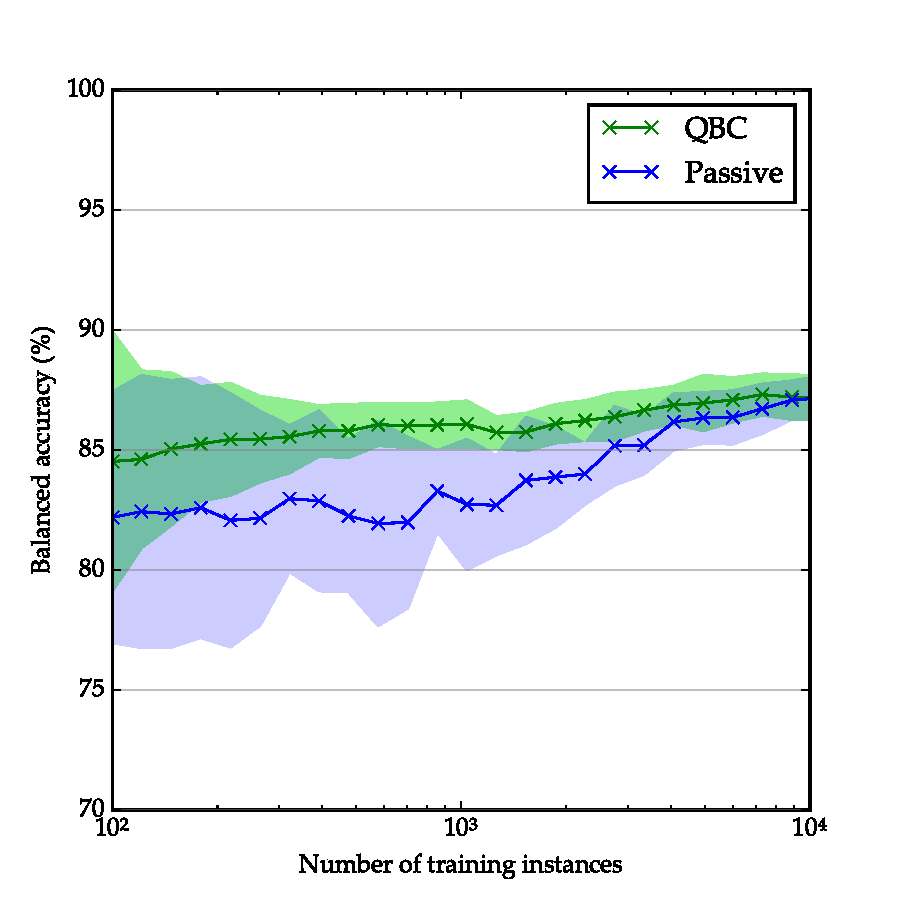
\includegraphics[width=0.8\textwidth]
            {images/experiments/rgz_qbc.pdf}
        \caption{Logistic regression trained on the \citeauthor{norris06}
            labels with different amounts of training data and two different
            query strategies.}
        \label{fig:rgz-qbc}
    \end{figure}

    We tested QBC active learning on the galaxy classification task described in
    Chapter \ref{cha:cross-identification}, comparing QBC to passive (i.e.
    random) selection as a query strategy.

    We used a committee of 20 logistic regression classifiers for the QBC test.
    Each was presented with 75\% of the known labels at random, stratified by
    the labels.

    For the passive test, we sampled 100 galaxies at random (stratified by the
    labels) and trained a logistic regression classifier on these. We then drew
    a batch of new labels, added these to the existing label set, and then
    retrained the classifier. This was repeated until the classifier had seen
    the entire training set ($10^4$ labels). The process for testing QBC was
    identical, except that instead of drawing new labels at random, the new
    labels were drawn in order of highest to lowest disagreement of the
    committee.

    After running the experiment, we observed that QBC outperformed passive
    selection. We hypothesised that this was because querying at random ignores
    the fact that there are far more negative examples than positive examples in
    the galaxy classification task. By this hypothesis, QBC would perform
    comparably to sampling from the set of positive examples and the set of
    negative examples at equal rates. To test this, we ran a third test with a
    random sampler that accounted for class imbalance. We found that this third
    test performed similarly to QBC.

    All three tested querying strategies are plotted in Figure
    \ref{fig:rgz-qbc}.

\section{Active Learning on Crowds}
\label{sec:active-learning-on-crowds}
    
    Traditional active learning assumes that we have access to one expert, who
    always issues correct labels. When labels are sourced from a crowd, these
    assumptions no longer hold: the crowd are non-experts and can give incorrect
    labels \citep{mozafari12,yan11}, and there are multiple labellers with
    different accuracies \citep{yan11}. We can now ask questions deeper than
    simply ``which label should I request?'' --- we can, for example, ask
    ``which labeller should I ask?'', or ``do I need to re-request this
    label?''.

    \citet{yan11} apply the \citet{yan10} model (Section \ref{sec:yan}) to the
    problem of active learning from crowds. We remind the reader that this model
    consists of a label model $p(z | \vec x)$ and a data-dependent labeller
    model $p(y_t | \vec x, z)$, where $\vec x$ is an instance, $y_t$ is the
    label assigned by labeller $t$, and $z$ is the groundtruth label. To extend
    this model into active learning, \citeauthor{yan11} introduce a query
    strategy where not only an instance is requested, but a specific labeller.

    First, uncertainty sampling is used with the label model to choose an ideal
    point to query. With logistic regression (Equation \ref{eq:raykar-logreg}),
    the decision boundary between positive and negative labels is a hyperplane
    $\vec w^T \vec x = 0$; uncertainty sampling would choose to query the point
    nearest (or on) this hyperplane. The labeller and instance to query are then
    chosen as solutions to the following optimisation problem:
    \begin{align*}
        \text{minimise}_{\vec x, t}\ & \eta_t(\vec x)\\
        \text{s.t. } & \vec w^T \vec x = 0.
    \end{align*}
    Intuitively, we query the instance on the decision hyperplane with the least
    noisy labeller. While this instance may not actually exist in our pool, we
    simply choose the instance closest to it (i.e. using Euclidean distance).

    This method has similar drawbacks to the \citeauthor{yan10} passive learning
    method described in Chapter \ref{cha:ml}: the number of parameters grows
    large with large numbers of annotators, and the expectation-maximisation
    algorithm only converges to a local minimum. In our implementation, training
    was also quite slow, meaning online active learning may be impractical. It
    also does not account for the possibility of relabelling instances.

    \citet{mozafari12} suggest an approach similar to uncertainty sampling, with
    uncertainty computed using a bootstrap method. A full description of this
    method is beyond the scope of this thesis. Instead, we look at the approach
    they take to handle noise. Noting that crowds may perform worse on some
    subsets of the data than other subsets, \citeauthor{mozafari12} solve an
    integer linear program to compute the redundancy required for different
    subsets of the instance pool. First, they partition the data, then estimate
    the probability of obtaining a correct crowd label for each partition. This
    estimation is accomplished by querying the crowd on a sample of instances
    from each partition. The estimated probability is then used to compute the
    redundancy required. For full details, we refer the reader to the paper
    \citep{mozafari12}.

\section{Active learning for Radio Galaxy Zoo}
\label{sec:ideal-experiment}
    
    Radio Galaxy Zoo \citep{banfield15} is a domain where active learning could
    be very useful. There are many more radio galaxies to classify than there
    are volunteers, so making the best use we can of their labels is
    particularly important.

    Applying active learning to the task that Radio Galaxy Zoo presents to their
    volunteers is non-trivial. Volunteers first choose which radio components
    are associated with the same AGN, and then decide where this AGN is located
    on an infrared image. Even ignoring the radio components problem, the
    position is a real-valued vector label, rather than a binary label. In this
    thesis, we have cast the cross-identification as a binary classification
    problem, converting these real-valued positions into binary labels by
    assigning a $1$ to the closest galaxy and $0$ to all other galaxies. This
    should still work for active learning, but there is no obvious way to
    develop a query strategy.

    Volunteers are presented with an image of radio object to label, so a query
    strategy must choose radio objects to present. Methods like uncertainty
    sampling have no clear application here: How do we convert from
    uncertainties in our classifications of neighbouring galaxies into an
    uncertainty for a radio object? We may be able to perform this aggregation
    by a number of methods, such as summing, averaging, or maximising the
    uncertainties. We could even aggregate using something like entropy, looking
    at the distribution of uncertainties of galaxies in the image. The choice is
    not obvious and an experiment is required. While we do not perform such an
    experiment in this thesis, we will suggest one at the end of this section.

    Query-by-committee may generalise to Radio Galaxy Zoo. We could label radio
    objects by considering nearby galaxies and classifying them using our
    methods from Chapter \ref{cha:cross-identification}, then selecting the
    galaxy with the most certain classification as the host galaxy of the radio
    object. Multiple classifiers could be used to perform this selection, and
    the percentage disagreement on the location of the host galaxy would then
    indicate the uncertainty associated with the radio object. However, this
    method would likely find radio objects that are intrinsically hard to
    cross-identify rather than radio objects where labelling would give high
    information gain. An example of this would be a compact radio object with
    multiple potential host galaxies very close to its centre. Cross-identifying
    such an object is usually very easy --- the galaxy closest to the centre is
    most likely to be the host galaxy --- but if there are multiple galaxies
    equidistant from the centre then a committee of classifiers will likely
    choose equally between them, resulting in high disagreement. In preliminary
    experiments with using QBC for this task, we found exactly this behaviour.

    An ideal experiment for active learning for Radio Galaxy Zoo would compare
    different generalisations of uncertainty sampling to QBC and passive
    sampling. In contrast to our approach to the cross-identification problem,
    instances would be radio objects rather than galaxies. Radio objects would
    be drawn using the different query strategies. The results of queries would
    come from an expert catalogue such as the \citeauthor{norris06} catalogue.
    The resulting labels would then be used to train a classifier. Training is
    possible using our methods by assigning all nearby galaxies a positive or
    negative label based on the result of the query, in a very similar way to
    how we converted the \citeauthor{norris06} and \citeauthor{fan15}
    cross-identifications into label sets. There is a clear problem of scale ---
    how large a radius around the radio object do we consider ``nearby''? ---
    and there is no clear solution to this problem.

    After such an experiment was used to determine good query strategies, the
    approach would need to be extended to work with the crowd. Queries would now
    be sent to a simulated crowd with realistic (i.e. Radio Galaxy Zoo
    volunteer-like) noise. This is a much harder problem to solve: One must now
    consider the problem of relabelling, label noise, and so on. Inspiration for
    such methods could likely be drawn from \citet{mozafari12}, as their
    partitioning approach is similar to that chosen by \citet{banfield15} for
    the Radio Galaxy Zoo (where the partitions are compact and complex radio
    objects).

    Reviewing these suggested experiments, it is clear that active learning for
    Radio Galaxy Zoo is a very hard problem to solve! As such, these experiments
    were beyond the scope of this work, but we hope that our classification
    methods may be applied in an aggregate way to radio objects in future work.

\section{Active Learning for Citizen Science}
\label{sec:al-citizen-science}
    
    Thus far, we have taken the word ``crowdsourcing'' to mean any scenario
    where there are multiple labellers. This conflates a number of arguably
    different scenarios: we may have multiple experts, multiple non-experts with
    domain knowledge, multiple non-experts without domain knowledge, and so on.
    The literature often does not disambiguate. \citet{raykar10} consider the
    problem of multiple experts who disagree; \citet{yan10} and
    \citet{mozafari12} consider crowdsourcing using a platform such as Amazon
    Mechanical Turk, where non-experts are paid to label data on a per-label
    basis. \citet{nguyen15} consider a hybrid scenario where we have access to
    both non-experts \emph{and} experts.

    The specific scenario we are interested in is citizen science, where
    volunteers interested in science contribute to labelling scientific data,
    typically through web interfaces like Galaxy Zoo \citep{lintott11}. With the
    rise of internet usage and the amount of available data throughout
    scientific disciplines, citizen science is steadily increasing in popularity
    and impact \citep{marshall15}. We believe that citizen science is a
    crowdsourcing scenario unlike those presented in existing literature, and as
    such, breaks assumptions often made by active learning methods that operate
    on crowds.

    There is a key difference between citizen science and paid crowdsourcing: In
    citizen science, we cannot choose our labellers. Using a paid crowdsourcing
    platform, we have some degree of freedom over who we query; this is (for
    example) the assumption made in \citet{yan11} and the crux of their methods.
    We can choose the best labeller and the best instance to query. In citizen
    science, volunteers request labels from us.

    It may also be difficult to estimate the accuracies of individual
    volunteers, for a number of reasons. These volunteers may be anonymous, and
    identifying which labels were assigned by the same individual may be
    impossible. Indeed, Radio Galaxy Zoo reports that 27\% of their labels come
    from anonymous volunteers. Another factor to consider is that a large number
    of labels in citizen science come from volunteers who only label a few
    instances. This means that trialling volunteers on a ``gold standard'' of
    instances with known groundtruth is impractical: If we tested every
    volunteer on a few known instances, then for many volunteers, the known
    instances would be all that they label! \citet{marshall15} highlight this
    with respect to Galaxy Zoo 2. They note the importance of designing projects
    for both recurring and new volunteers, citing the significant contributions
    of both groups. A visualisation of Galaxy Zoo 2 volunteer contributions is
    reproduced here in Figure \ref{fig:galaxy-zoo-2-volunteer-distribution}.

    Finally, citizen science tends to involve a very large number of labellers:
    Galaxy Zoo has involved several hundred thousand volunteers
    \citep{marshall15}; Radio Galaxy Zoo has over 2000 volunteers involved with
    just the ATLAS--CDFS observations that we have looked at in this thesis. For
    contrast, \citet{raykar10}, on whose methods we based our own crowd
    experiments, used 5 labellers for most of their experiments (with one
    experiment with 164 labellers); \citet{mozafari12} and \citet{yan11} both
    tested their methods with 3--5 labellers. The large number of labellers
    involved in practical citizen science raises many challenges. Estimating
    labeller accuracies is very difficult for large numbers of labellers as the
    number of model parameters is often tied to the number of labellers.
    Additionally, the label matrix $y_{t, i}$ is sparse: Most labellers have not
    labelled most instances.

    \begin{figure}
        \centering
        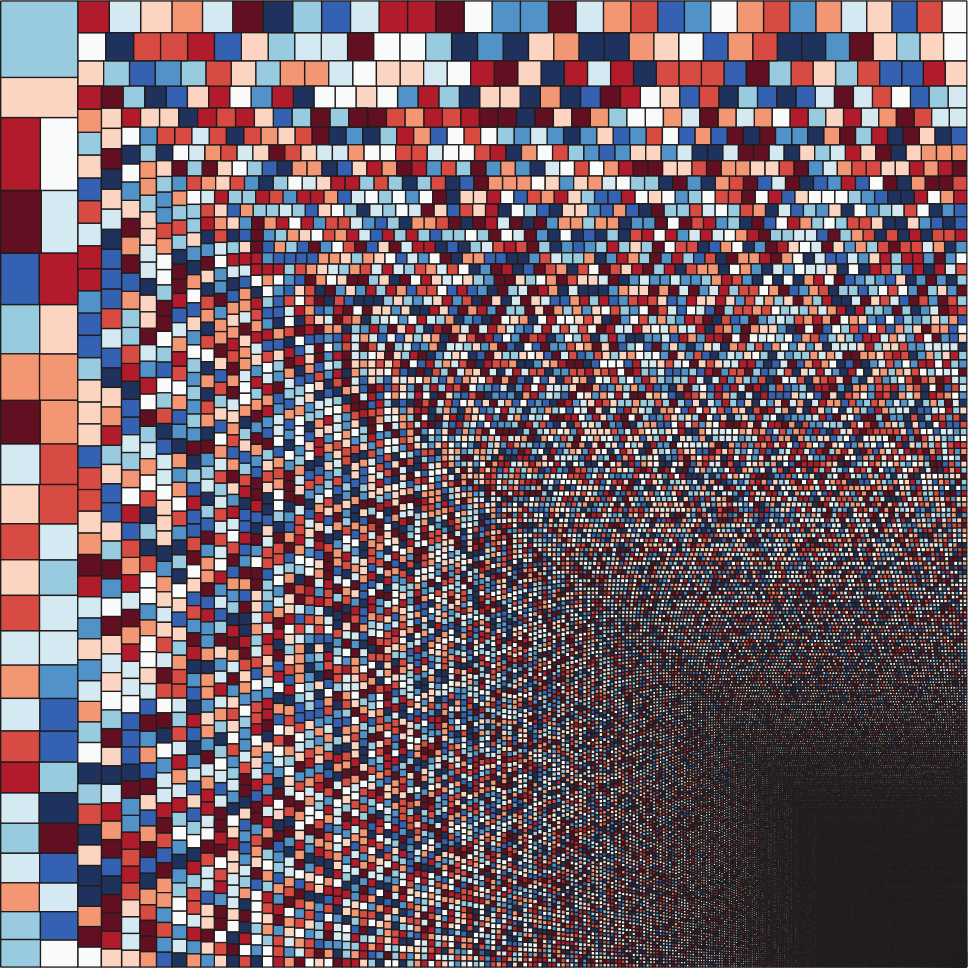
\includegraphics[width=0.8\textwidth]{images/galaxyzoovolunteers}
        \caption{Label contributions from volunteers in Galaxy Zoo 2. Each
            square represents a single user, with the area of the square
            proportional to the number of instances labelled by that user.
            \emph{Image: K. Willett. Reproduced from \citet{marshall15}.}}
        \label{fig:galaxy-zoo-2-volunteer-distribution}
    \end{figure}
